\chapter{Related Work}
\label{ch:Related-Work}

This chapter introduces and explains terms and concepts which will be used throughout the thesis. Thus, this section can be used as a reference guide to fill in any gaps and to understand the relationships between the individual concepts better.

\section{Introduction to Digital Signal Processing}
\label{sec:Intro-DSP}

This section introduces the fundamentals of \gls{DSP}, which will be used repeatedly in the following chapters, either to reason or to describe some behaviour. 
\newline
\newline
What exactly is \gls{DSP}? \gls{DSP} is to take real-world signals like voice, audio, video, temperature, pressure, or position that have been digitized and then mathematically manipulate them. A \gls{DSP} is designed for performing mathematical functions like \textit{add}, \textit{subtract}, \textit{multiply} and \textit{divide} very quickly.
\newline
\newline
Signals need to be processed so that the information that they contain can be displayed, analyzed, or converted to another type of signal that may be of use. In the real-world, analogue products detect signals such as sound, light, temperature or pressure and manipulate them. Converters such as an \gls{ADC} then take the real-world signal and turn it into the digital format of 1's and 0's. From here, the \gls{DSP} takes over by capturing the digitized information and processing it. It then feeds the digitized information back for use in the real world. It does this in one of two ways, either digitally or in an analogue format by going through a \gls{DAC}. All of this occurs at very high speeds.\footnotemark

\footnotetext{\href{https://www.analog.com/en/design-center/landing-pages/001/beginners-guide-to-dsp.html}{analog.com/en/design-center/landing-pages/001/beginners-guide-to-dsp.html}}

\subsection{Amplitude}
\label{sub:Amplitude}

The amplitude of a periodic variable is the measure of how far, and in what direction, that variable differs from zero. Thus, signal amplitudes can be either positive or negative. The figure \ref{fig:Amplitude-Wavelenght} illustrates the amplitude with variable $y$. 
\newline
\newline
The distance from the top of one peak to the bottom of another is called \textit{peak-to-peak amplitude}. Another way to describe peak-to-peak amplitude is to say that it is the distance between the maximum positive value and the maximum negative value of a wave. In figure \ref{fig:Amplitude-Wavelenght}, the peak-to-peak amplitude of the wave would be $2y$.

\subsection{Magnitude}
\label{sub:Magnitude}

The magnitude of a periodic variable is the measure of how far, regardless of direction, its quantity differs from zero. So magnitudes are always positive values. Occasionally, in the literature of digital signal processing, the term magnitude is referred to as the absolute value. In figure \ref{fig:Amplitude-Wavelenght}, the magnitude of the wave would be $|y|$.

\subsection{Wavelength}
\label{sub:Wavelength}

The wavelength is the length of a single cycle of a wave, as measured by the distance between one peak of a wave and the next. In figure \ref{fig:Amplitude-Wavelenght} the wavelength is designated as the variable $\lambda$.

\begin{figure}[htbp]
	\centering
	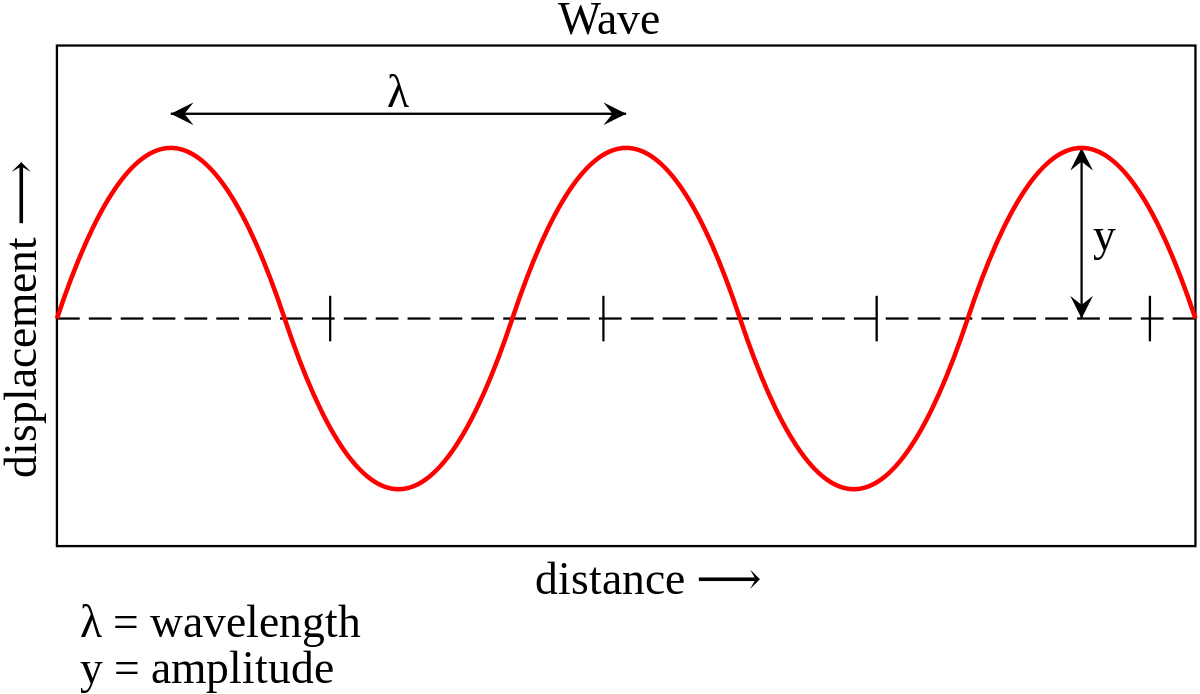
\includegraphics[scale=0.25]{baa-documentation/img/Amplitude.png}
	\caption[Amplitude and wavelength illustrated]{Amplitude and wavelength \footnotemark}
	\label{fig:Amplitude-Wavelenght}
\end{figure}
\footnotetext{\href{https://en.wikiversity.org/wiki/Amplitude}{\nolinkurl{en.wikiversity.org/wiki/Amplitude}}}

\subsection{Sampling}
\label{sub:Sampling}

Sampling is the first step to convert an analogue signal to a digital one. Firstly the signal has to be sampled using a device called an \gls{ADC}. The \gls{ADC} will measure the signal at rapid intervals, and these measurements are called samples. It will output a digital signal proportional to the amplitude of the analogue signal at that same instant.

\subsection{Aliasing}
\label{sub:Aliasing}

Aliasing is a special effect that can happen when the speed of samples taken from the analogue signal is to low compared to the actual analogue signal, otherwise known as frequency. Aliasing is due to the fact that the actual signal is changing so rapidly between sampling instants, that this rapid movement is not visible in the sampled signal. The sampled signal appears to be a lower frequency signal compared to the actual signal.

\subsection{Quantization}
\label{sub:Quantization}

Quantization is the process of mapping input values from a large continuous set to output values in a smaller collection, with a finite number of elements. Not all input values can be represented in the finite set, so the values have to be mapped to an existing number (quantized value) in it. This is usually done by rounding or truncation. The difference between an input value and its quantized value is referred to as quantization error. A device or algorithmic function that performs quantization is called a quantizer. An \gls{ADC} is an example of a quantizer.

\subsection{Sampling Frequency and Resolution}
\label{sub:Sampling-Frequency-Resolution}

The sampling frequency or sampling rate, given in \gls{Hz}, of an audio signal, determines the resolution of the audio sample. The sampling frequency states how many samples (amplitudes \ref{sub:Amplitude}) were captured for each second of the signal. Each one of these samples also has a resolution, given in bits, which determines how detailed audio waveforms are. This resolution is also referred to as bit depth. The higher the sampling rate, the higher the resolution of the signal. When recording music or many types of acoustic events, audio waveforms are typically sampled at 44.1 \gls{kHz} (CD), 48 \gls{kHz}, 88.2 \gls{kHz}, or 96 \gls{kHz}. Sampling rates higher than about 50 \gls{kHz} to 60 \gls{kHz} cannot supply more usable information for human listeners. Early professional audio equipment manufacturers chose sampling rates in the region of 40 to 50 \gls{kHz} for this reason.

\subsection{Nyquist–Shannon sampling theorem}
\label{sub:Nyquist–Shannon}

This theorem was introduced to prevent the \nameref{sub:Aliasing} phenomenon and give some rule or convention to sampling. The Nyquist-Shannon sampling theorem implies, to sample more than twice as fast as the signal to convert.
\newline
\newline
Whenever a sampled signal is given, there is no certainty that the signal represents the analogue one. However, if the signal was sampled at more than twice the frequency of the signal, then the sampled signal will accurately represent the same frequency as the actual signal ere sampling. The critical frequency which the signal must not ever exceed, which is precisely one half of the sampling frequency, is called the Nyquist frequency.

\subsection{Noise}
\label{sub:Noise}

Noise is any unwanted signal distorting the original signal. Given a speech signal with amplitude $s(n)$, where $n$ is the sample index, noise is any other signal, $w(n)$ which interferes with the speech. The noisy speech signal $u(n)$ is defined with equation \ref{eq:Noise-Added}.

\myequations{Noise added to a signal}
\begin{equation}
    \centering
    u(n) = s(n) + w(n)
    \label{eq:Noise-Added}
\end{equation}

\subsection{Time domain}
\label{sub:Time-Domain}

The time-domain refers to the analysis of mathematical functions of signals with respect to time. A time-domain graph shows how a signal changes with time. 
\newline
\newline
A wave plot is a visual representation of this domain. The y-axis of such visualisation represents the \nameref{sub:Amplitude} (loudness) of the sound wave, whereas the x-axis represents the time. If the amplitude is equal to zero, it represents silence. Such a representation is shown in figure \ref{fig:Waveplot-Time-Domain}.

% TODO - create own wave plot
\begin{figure}[htbp]
	\centering
	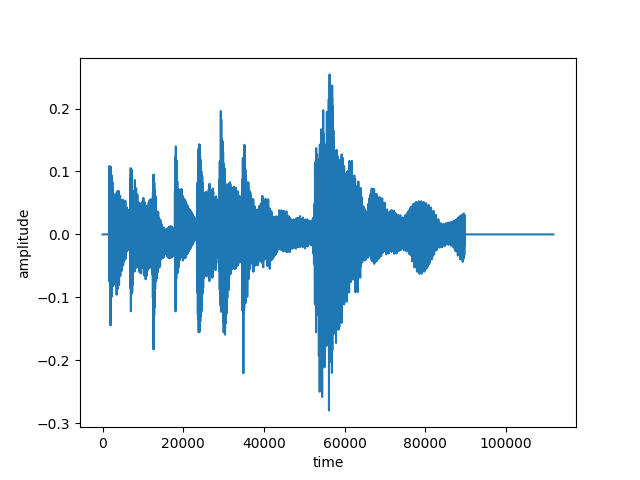
\includegraphics[scale=0.6]{baa-documentation/img/Waveplot-time-domain.png}
	\caption[Time-domain illustrated in wave plot]{Time-domain illustrated in wave plot \footnotemark}
	\label{fig:Waveplot-Time-Domain}
\end{figure}
\footnotetext{\href{https://stackoverflow.com/questions/43835055/plotting-audio-from-librosa-in-matplotlib}{\nolinkurl{stackoverflow.com/questions/43835055/plotting-audio-from-librosa-in-matplotlib}}}

\subsection{Frequency domain}
\label{sub:Frequency-Domain}

The frequency-domain refers to the analysis of mathematical functions or signals with respect to frequency. A frequency-domain graph shows how much of the signal lies within each given frequency band over a range of frequencies. 
\newline
\newline
A given function or signal can be converted between the time and frequency domains with a pair of mathematical operators. The most used operation is the Fourier Transformation, which will be explained in further detail in section \ref{sub:Fourier-Transform}.

\subsection{Fourier Transform}
\label{sub:Fourier-Transform}

\gls{FT} is a mathematical concept that can convert a continuous signal from \fullref{sub:Time-Domain} to \fullref{sub:Frequency-Domain}. It decomposes a signal into its constituent frequencies along with the magnitude of each frequency.

\subsubsection{Fast Fourier Transform}
\label{subsub:Fast-Fourier-Transform}

\gls{FFT} is a mathematical algorithm that calculates \gls{DFT} of a given sequence. The only difference between \gls{FT} and \gls{FFT} is, that \gls{FT} considers a continuous signal while \gls{FFT} takes a discrete signal as input. \gls{DFT} converts a sequence, a discrete signal, into its frequency constituents just like \gls{FT} does for a continuous signal. It is important to note that due to that transformation, the time information of the audio signal will be lost.

\subsubsection{Short Time Fourier Transform}
\label{subsub:Short-Time-Fourier-Transform}

\subsection{Spectrogram}
\label{sub:Spectrogram}

A spectrogram is a visual representation of the frequency domain. More precisely it represents the spectrum of frequencies of a signal as it varies with time. The x-axis represents the time, the y-axis represents the frequencies, and the colours represent the magnitude of the observed frequency at a particular time. Bright colours represent powerful frequencies. Thus every spectrogram represents three domains: time, frequency and magnitude.
\newline
\newline
To create a spectrogram, the audio signal is broken down into smaller frames (windows), and for each one, the \gls{DFT} or \gls{FFT} will be calculated. The resulting frequencies of each window will represent the time. It is important to note that the windows should overlap each other, not to lose any frequency. Typical window sizes are 20 to 30ms, but this size highly depends on the task to solve. The figure \ref{fig:Spectrogram} show an example of such a spectrogram.

% TODO - create own spectrogram
\begin{figure}[htbp]
	\centering
	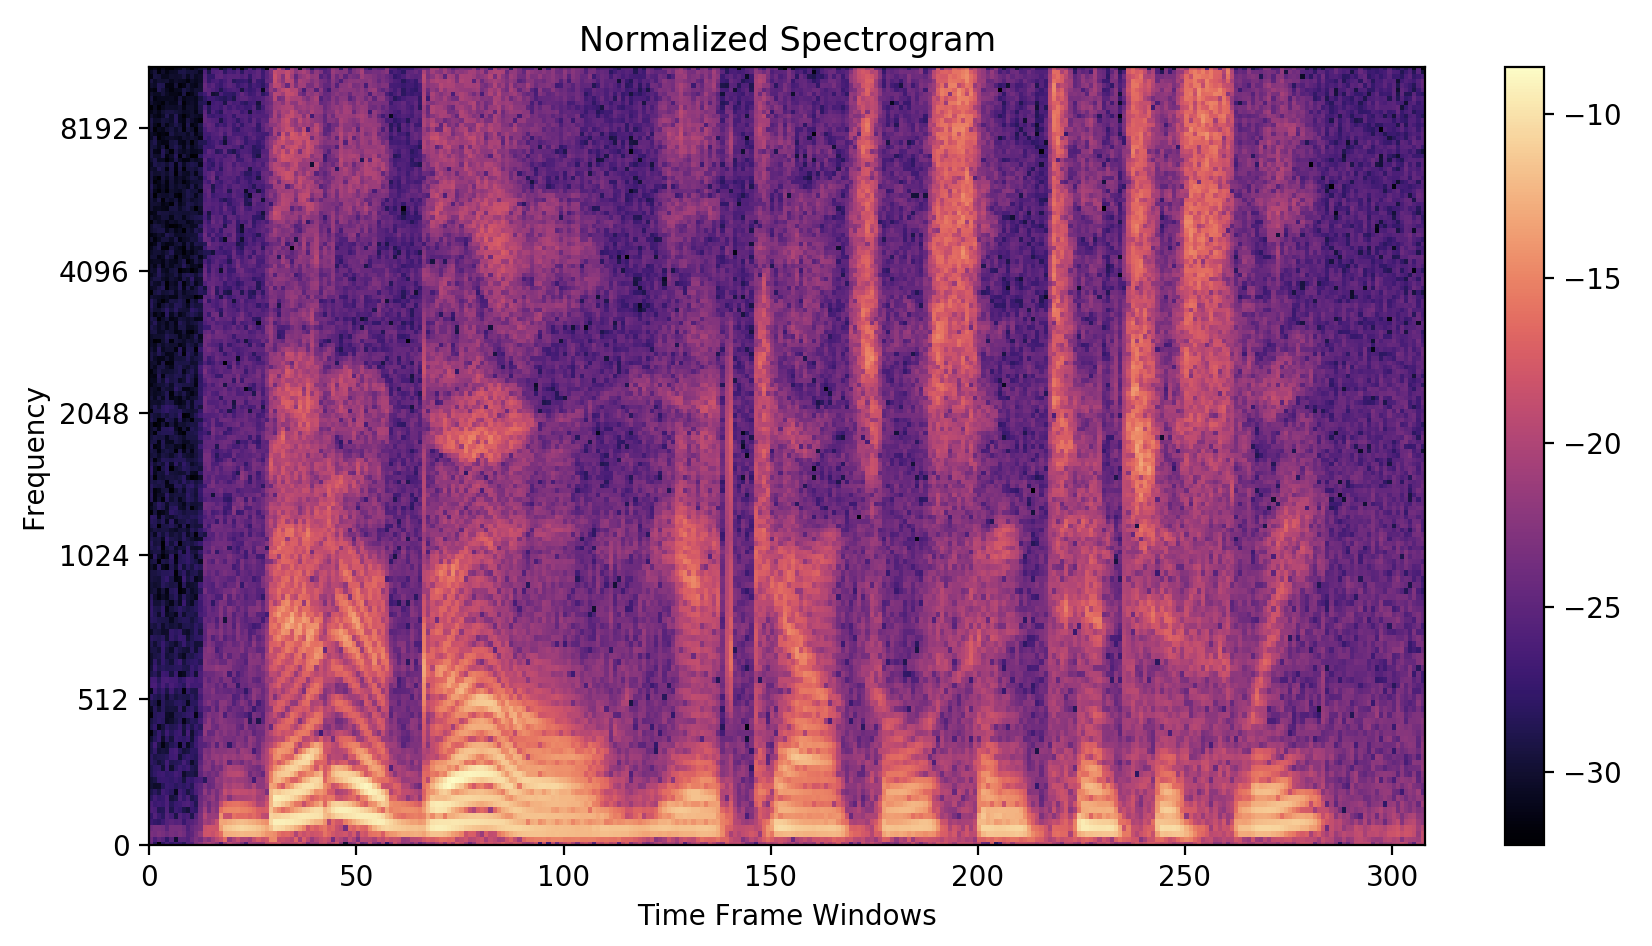
\includegraphics[scale=0.2]{baa-documentation/img/Spectrogram.png}
	\caption[Example of a spectrogram]{Example of a spectrogram \footnotemark}
	\label{fig:Spectrogram}
\end{figure}
\footnotetext{\href{https://towardsdatascience.com/understanding-audio-data-fourier-transform-fft-spectrogram-and-speech-recognition-a4072d228520}{\nolinkurl{towardsdatascience.com/understanding-audio-data-fourier-transform-fft-spectrogram-and-speech-recognition-a4072d228520}}}

\subsection{Mel Spectogram}
\label{sub:Mel-Spectogram}

% TODO - 2/3 sites

\subsection{$\mu$-law Transformation}
\label{sub:Mu-Law-Transformation}

\subsection{LibROSA}
\label{sub:Librosa}

LibROSA is a python package for music and audio analysis. It provides the building blocks necessary to create music information retrieval systems.\footnote{\url{https://librosa.github.io/librosa/}}

\section{Introduction to Neural Nets}
\label{sec:Intro-NN}

In this section, technical concepts are explained in more detail, which was used in the thesis. These concepts are mostly very complex and are, therefore only touched upon so that the further conclusions of this work can be understood comprehensibly.

\subsection{Neural Nets}
\label{sub:Neural-Nets}

\subsection{Convolutional Neural Nets}
\label{sub:Convolutional-Neural-Nets}

\subsection{Gated Linear Unit}
\label{sub:Gated-Linear-Unit}

\subsection{Tensorflow}
\label{sub:Tensorflow}

TensorFlow is an end-to-end open source platform for machine learning. It has a comprehensive, flexible ecosystem of tools, libraries and community resources that lets researchers push the state-of-the-art in \gls{ML} and developers easily build and deploy \gls{ML} powered applications. \footnote{\url{https://www.tensorflow.org/}}

\section{State of the art}
\label{sec:State-of-art}

\subsection{Word2Vec}
\label{sub:word2wec}

\subsection{Triplet Loss}
\label{sub:Triplet-Loss}

\section{Status in relation to project}
\label{sec:Status-Relation-Project}
